\documentclass[a4paper,12pt,hidelinks]{report}
\usepackage{graphicx}
\usepackage[parfill]{parskip}
\usepackage[backend=bibtex,style=ieee]{biblatex}
\usepackage{fancyhdr}
\usepackage[top=3cm,bottom=3cm,left=3cm,right=3cm,headheight=15pt]{geometry}
\usepackage{gentium}
\usepackage{titlesec}
\usepackage{placeins}
\usepackage{caption}
\usepackage{subcaption}
\usepackage{textcomp}
\usepackage[UKenglish]{isodate}
\usepackage{blindtext}
\usepackage{pdflscape}
\usepackage{tabularx}
\usepackage{longtable}

\usepackage[pdftex,pdfauthor={Dale Mark Peters (Student Number 120062861)},pdftitle={SE31520 Assignment Documentation | Aberystwyth University},pdfcreator={pdflatex}]{hyperref}

\title{SE31520 Assignment Report}
\author{Dale Mark Peters}
\graphicspath{{/home/dale/university/se31520/assignment/report/images/}}

\bibliography{bibliography}
\captionsetup{width=0.8\textwidth,font={small}}

\titleformat
{\chapter}
[block]
{\bfseries\huge}
{\thechapter}
{3ex}
{}
[]

\pagestyle{fancy}
\fancyhf{}
\lhead[LO]{\leftmark}
\rhead[RE]{\rightmark}
\cfoot{\thepage}
\begin{document}

\maketitle

\newgeometry{left=4cm,right=4cm}
\renewcommand{\abstractname}{Acknowledgements}
\begin{abstract}
\end{abstract}
\restoregeometry

\tableofcontents\newpage
\chapter{Introduction}
    This document it written to accompany the software I have written for the SE31520 (Developing Internet Based Applications) 2015-2016 assignment. In this
    document, I will describe the architecture and justify the design of my web application and RESTful APIs developed, and will then go on
    to explain the testing strategy used for my applications and give the results of the tests. Finally, I will give an evaluation of how well the requirements
    were met and how well I have done in the assignment.

    In this assignment, I was tasked with the design and implementation of a web application (My Alcohol Free Wines - from now on called MAF) that allows users to find the cheapest prices
    for the non-alcoholic wines they wish to buy. This had to be done by comparing the prices of one identical wine from two different suppliers and displaying the
    cheapest one in the MAF wines listing page. From the wines listings page, the idea was that they can then place their desired wines into their basket and place
    an order, where an `order' consists of sending the details of the purchase and the customer details to the relevant supplier via a RESTful request.

\chapter{Design/Architecture}
    \section{Data Structures}
    From the specification of the assignment and the system that needs to be implemented, some of the models that needed to be considered were clear. 
    These are detailed in this section.
    
    \subsection{Wine}
    Perhaps the most important of the data structures to be represented in the application is the products that the shop is selling to its customers (i.e.\ a
    particular bottle of wine). These are retrieved from two suppliers but will need to be stored in the MAF database to reduce the number of hits the application
    does on the data services and to improve the performance of MAF. Information stored about the products is as follows:
    \begin{itemize}
            \item \textbf{Short and long description} (String): Holds the title of the wine and the long description respectively. These will be textual.
            \item \textbf{Bottle Size} (String): I have made the assumption that this will be from a set of sizes (small, medium or large).
            \item \textbf{Price} (float): This could be decimalised with two decimal places, so a float representation is most appropriate.
            \item \textbf{Origin Country, Company and Grape Types} (String): Textual fields, so string is the best choice.
            \item \textbf{Vegetarian (boolean)}: This can either be true or false, so boolean is the best choice.
    \end{itemize}

    In addition to these attributes, I added a barcode attribute to the wine. While this wasn't specified in the specification, it was necessary to add 
    this to ensure that an identical product from different suppliers can be compared, even if they have different short descriptions or long descriptions.
    This is stored as a string to cover for cases where the barcode might begin with a 0.

    \section{Use Case Diagram}
    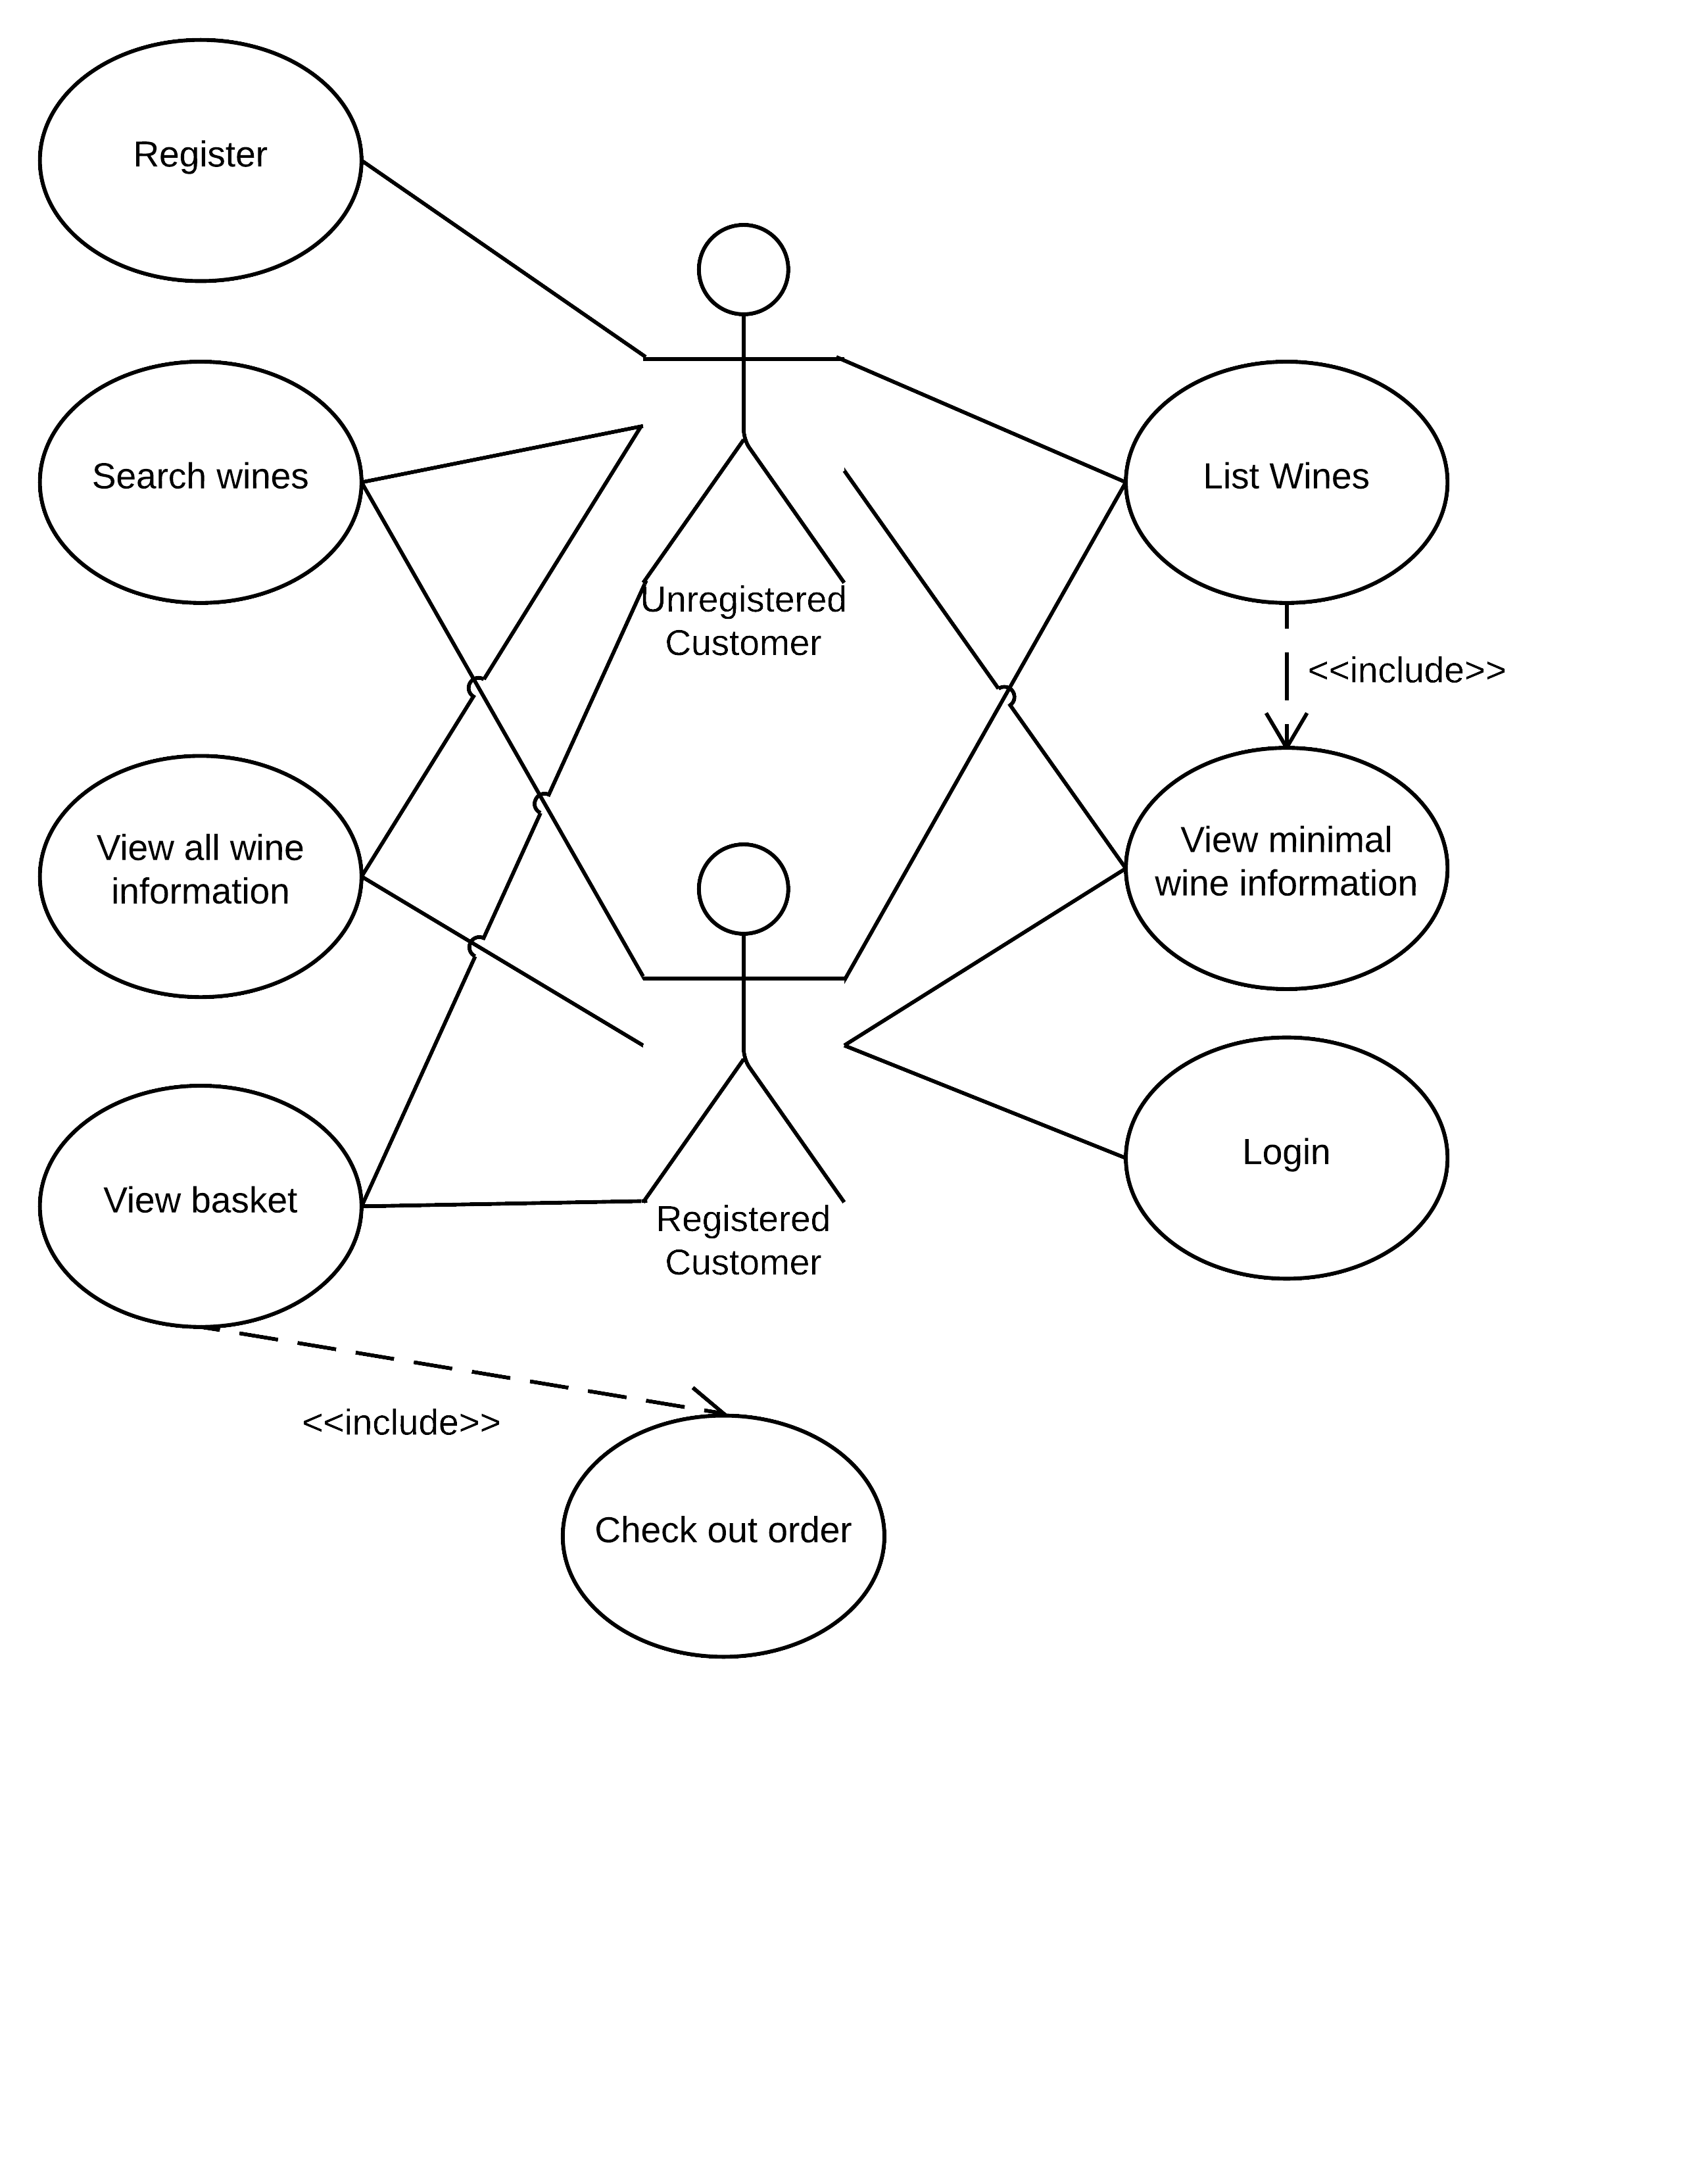
\includegraphics[scale=0.60]{use-case-diagram.png}

    \section{Architecture Diagram}
    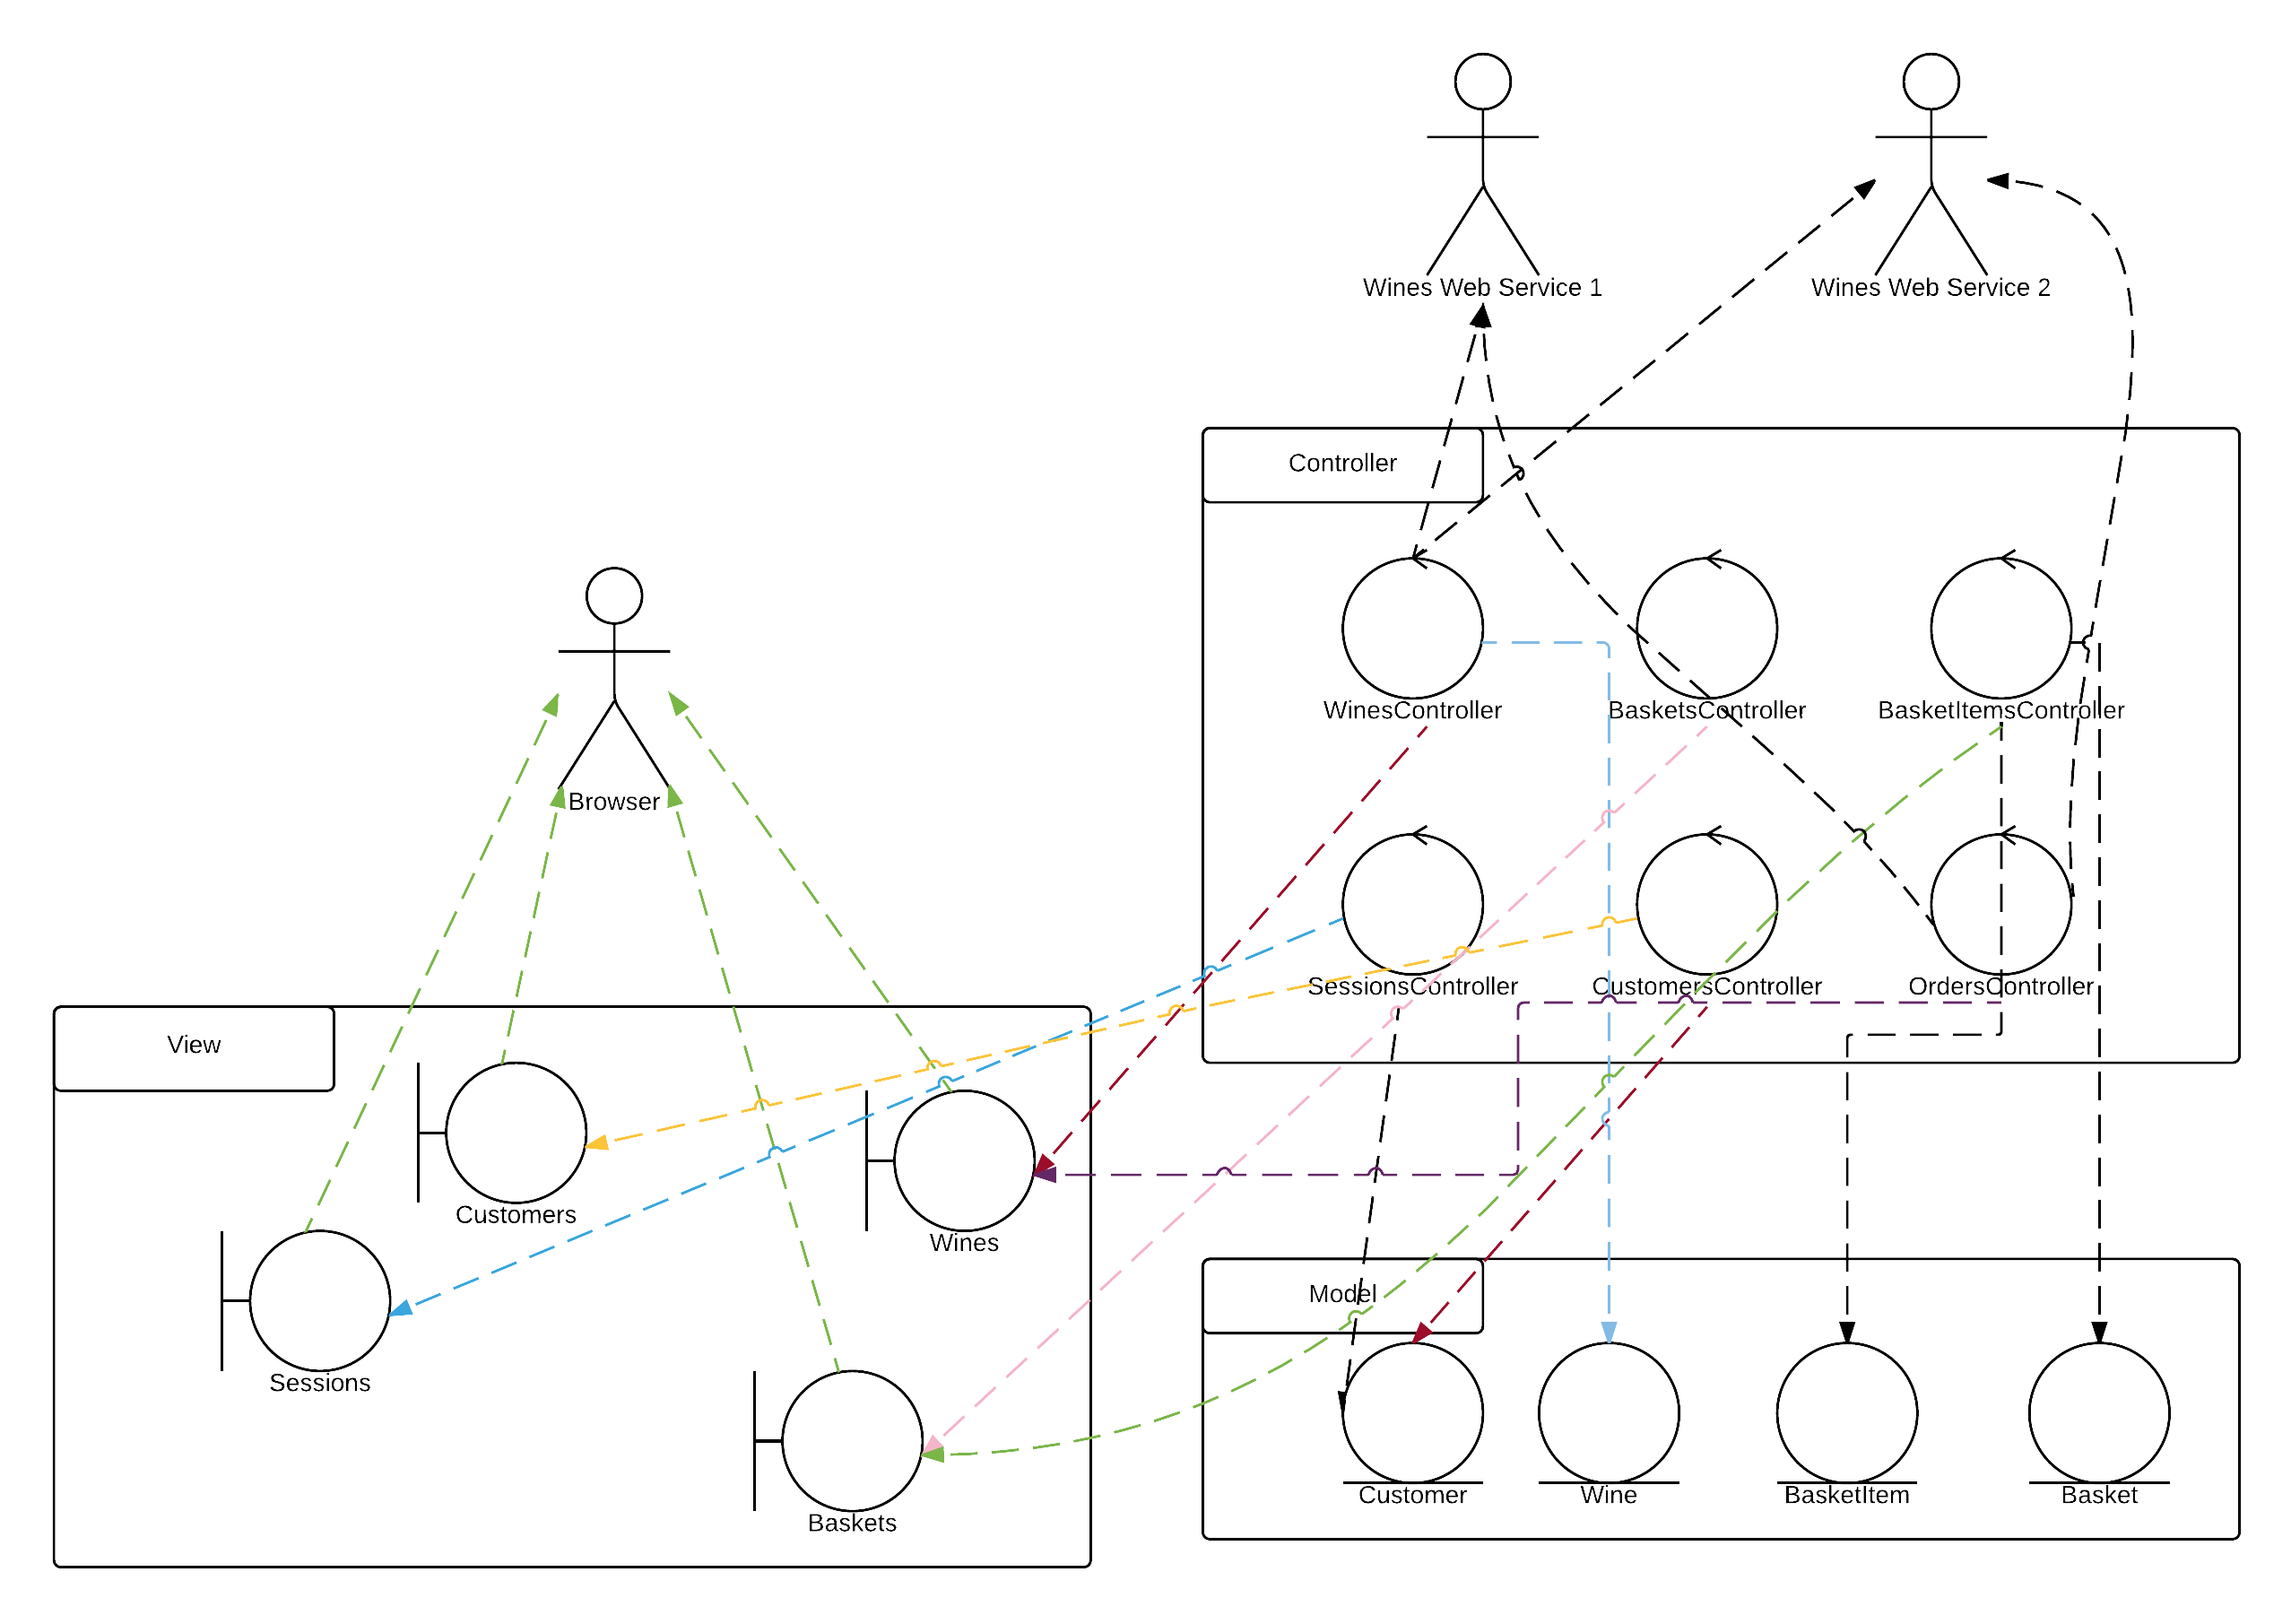
\includegraphics[width=\textwidth]{architecture-diagram.png}

    \section{My Alcohol Free Wines}
    \subsection{Routes}
    This section details the routes that are used in the application.


    \section{RESTful Supplier Web Services}
    As previously mentioned, another part of this assignment was to develop two external RESTful HTTP web services (the suppliers to MAF) which
    supply MAF with all the information on the wines they sell. They also needed to have the capability of receiving order details from MAF when the
    user clicks the checkout button in their cart.

    My two APIs use exactly the same implementation (identical code), and have a HTTP GET route (\url{http://localhost:5000/wines/} and \url{http://localhost:5001/wines/} 
    defined for the supply of wine information to MAF, and a HTTP POST route (\url{http://localhost:5000/orders/} and \url{http://localhost:5001/orders/}).
    Both of these supply and receive data in the form of JSON objects. The reason for this choice was because for each JSON object, there is significantly less
    text than XML and it is good enough for representing the simple nature of the data to be sent between the systems.

    The two services were written in Python, using the \textit{Flask} framework \cite{flask-framework}. I chose to implement these in Python because over my industrial 
    year, I gained experience in this language and it is one I feel confident in. It also didn't require me to write very much code for the web services, compared to the likes of
    Java, for example, so development time was minimal. Whilst I'd had experience in writing software in Python before, I'd never developed a RESTful API with Flask,
    so I had to follow a tutorial to help me with this \cite{flask-tutorial}. The orders sent to the server are not stored when received in this prototype, as this
    is not a requirement of the assignment. Rather, the orders are stored in memory when received. The wines are also stored in memory when the web service server is
    started. \textbf{STORE IN JSON FILE AND CHANGE THIS IF HAVE TIME}. If I had the time, I would have stored these in a separate JSON file and read this in when the service
    starts, so as to reduce the amount of text in the service code. The data in the two applications is different so that the two suppliers' prices can be compared.


\chapter{Testing}
    \section{Test Strategy}

    %\newpage
    \begin{landscape}
        \section{Test Results}
        \begin{center}
            \begin{longtable}{ |c|c|c|c|c|c|c|c| } 
                \hline
                \textbf{Test ID} & \textbf{Requirement} & \textbf{Description} & \textbf{Inputs} & \textbf{Expected Outputs} & \textbf{Actual Outputs} & \textbf{Pass/Fail} & \textbf{Comments}
                \\\hline\hline
                1 & FR1 & On list wines screen: Customer can see wines sold, listed in alphabetical order and paginated & Navigate to wines page & List of all wines sold by MAF & & & Comments\\ \hline
                1 & FR1 & On list wines screen: Customer can see wine picture, short description, bottle size, price and supplier & Navigate to wines page, look at information listed & All information displayed & & & Comments\\ \hline
                1 & FR1 & On list wines screen: Customer can see wine picture, short description, bottle size, price and supplier & Navigate to wines page, look at information listed & All information displayed & & & Comments\\
                1 & FR1 & On list wines screen: Customer can see wine picture, short description, bottle size, price and supplier & Navigate to wines page, look at information listed & All information displayed & & & Comments\\
                \hline
            \end{longtable}
        \end{center}
    \end{landscape}

    \blindtext
\chapter{Self Evaluation}
    \blindtext

\printbibliography

\end{document}
